\documentclass{if-beamer}

\usepackage[normalem]{ulem}

% --------------------------------------------------- %
%                  Presentation info	              %
% --------------------------------------------------- %
\title[Liczba Dedekinda]{Liczba Dedekinda}
\subtitle{Liczba monotonicznych funkcji boolowskich n-zmiennych}
\author{Jan Iwaszkiewicz}
\institute[MFI]{
  Wydział Matematyki, Fizyki i Informatyki\\
  Uniwersytet Gdański
}
\date{14 maja 2019}
% \logo{
% \includegraphics[scale=0.03]{flash_edit.png} % ZMIENIĆ
% }
\subject{OpenMP optymalizacja} % metadata

\graphicspath{{graphics/}}
% --------------------------------------------------- %
%                    Title + Schedule                 %
% --------------------------------------------------- %

\begin{document}

% \usebackgroundtemplate{%
%  \includegraphics[scale=0.42]{flash_edit.png}} 
\begin{frame}
  \titlepage
\end{frame}

\usebackgroundtemplate{} 
\begin{frame}{Plan prezentacji}
  \tableofcontents
\end{frame}

% --------------------------------------------------- %
%                      Presentation                   %
% --------------------------------------------------- %
\section{Wstęp i przypomnienie}
\begin{frame}{Wstęp - Richard Dedekind}

\begin{columns}

\begin{column}{0.6\textwidth}
\textbf{\exemple{Richard Dedekind}} niemiecki matematyk, uczeń Petera Gustava Dirichleta i Carla Friedricha Gaussa, przyjaciel Georga Cantora. Jego prace dotyczą głównie teorii liczb, algebry, teorii mnogości i analizy matematycznej.
\end{column}

\begin{column}{0.4\textwidth}

\begin{figure}
\centering
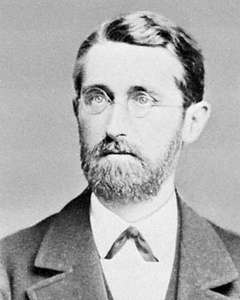
\includegraphics[scale=0.4]{richard.jpg}
\caption{Julius Wilhelm Richard Dedekind}
\end{figure}

\end{column}

\end{columns}
\blfootnote{\href{https://pl.wikipedia.org/wiki/Richard_Dedekind}{https://pl.wikipedia.org/wiki/Richard\_Dedekind}}
\end{frame}

\subsection{Liczba Dedekinda}
\begin{frame}{Liczba Dedekinda}
\textbf{\exemple{Liczbą Dedekinda}} możemy nazwać ilość elementów w zbiorze monotonicznych boolowskich funkcji o $k$-zmiennych (gdzie $ k \in [0, \infty) $). Taki zbiór będziemy określać jako \textbf{\exemple{$ M_{k}$}}.
\blfootnote{\href{https://en.wikipedia.org/wiki/Dedekind_number?fbclid=IwAR39NYrkpOReHVf0AXa4uhYPM6c0NrNvLLWMtGrG4LEkjDYPxUXIE4hLSU8}{Wikipedia - Dedekind number}}
\end{frame}

\subsection{Przypomnienie - funkcja boolowska}
\begin{frame}{Przypomnienie - funkcja boolowska}

\begin{block}{Definicja}
\centering
$ f: B^{k} \rightarrow B$
\linebreak
$ B = \lbrace 0, 1 \rbrace $
\linebreak
$ k \in [0,\infty) $
\linebreak\linebreak
$B^{k} \in 2^{k}$ elementów oraz $2^{2^{k}}$ funkcji boolowskich z $k$-zmiennymi
\end{block}

\begin{block}{Przykład}
\centering
$B^{0} = \lbrace 0, 1 \rbrace$
\linebreak
$B^{1} = \lbrace 00, 01, 10, 11 \rbrace$
\linebreak
$B^{2} = \lbrace 0000, 0001, 0010, 0011, 0100, 0101, ... \rbrace$
\end{block}
\blfootnote{\href{https://en.wikipedia.org/wiki/Boolean_function}{https://en.wikipedia.org/wiki/Boolean\_function}}
\end{frame}

\subsection{Przypomnienie - monotoniczność}
\begin{frame}{Przypomnienie - monotoniczność}

\begin{block}{Definicja}
\centering
Porządek relacji w $B$:
\linebreak\linebreak
$ 0 \leqslant 0, 0 \leqslant 1, 1 \leqslant 1 $
\linebreak\linebreak
Oraz częściowy porządek w $B^{k}$:
\linebreak\linebreak
$ x = (x_{1}, ... , x_{k}), y = (y_{1}, ... , y_{k}) $ 
\linebreak\linebreak
$ x \leqslant y $ dla $ x_{i} \leqslant y_{i}, i \in [1, k] $
\linebreak\linebreak
Zatem funkcja g jest monotoniczna gdy:
\linebreak\linebreak
$ x \leqslant y \Rightarrow g(x) \leqslant g(y) $
\end{block}

\end{frame}

\subsection{Przypomnienie - konkatenacja dwóch funkcji}
\begin{frame}{Przypomnienie - konkatenacja dwóch funkcji}

\begin{block}{Twierdzenie}
\centering
Konkatenacja dwóch funkcji monotonicznych tworzy również funkcję monotoniczną. 
\end{block}
\begin{flushleft}
Przykłady (nie)monotonicznych funkcji:
\begin{large}
\linebreak\linebreak
$ 0 \cdot 1 \rightarrow 01 $
\linebreak\linebreak
$ 1 \cdot 0 \nrightarrow 10 $, brak spełnionego warunku
\linebreak\linebreak
$ 0101 \cdot 1111 \rightarrow 0101 1111 $
\end{large}
\end{flushleft}
\end{frame}

\section{Algorytmy}

\subsection{Wizualizacja kostek}

\begin{frame}{Wizualizacja kostek}

\begin{figure}
\centering
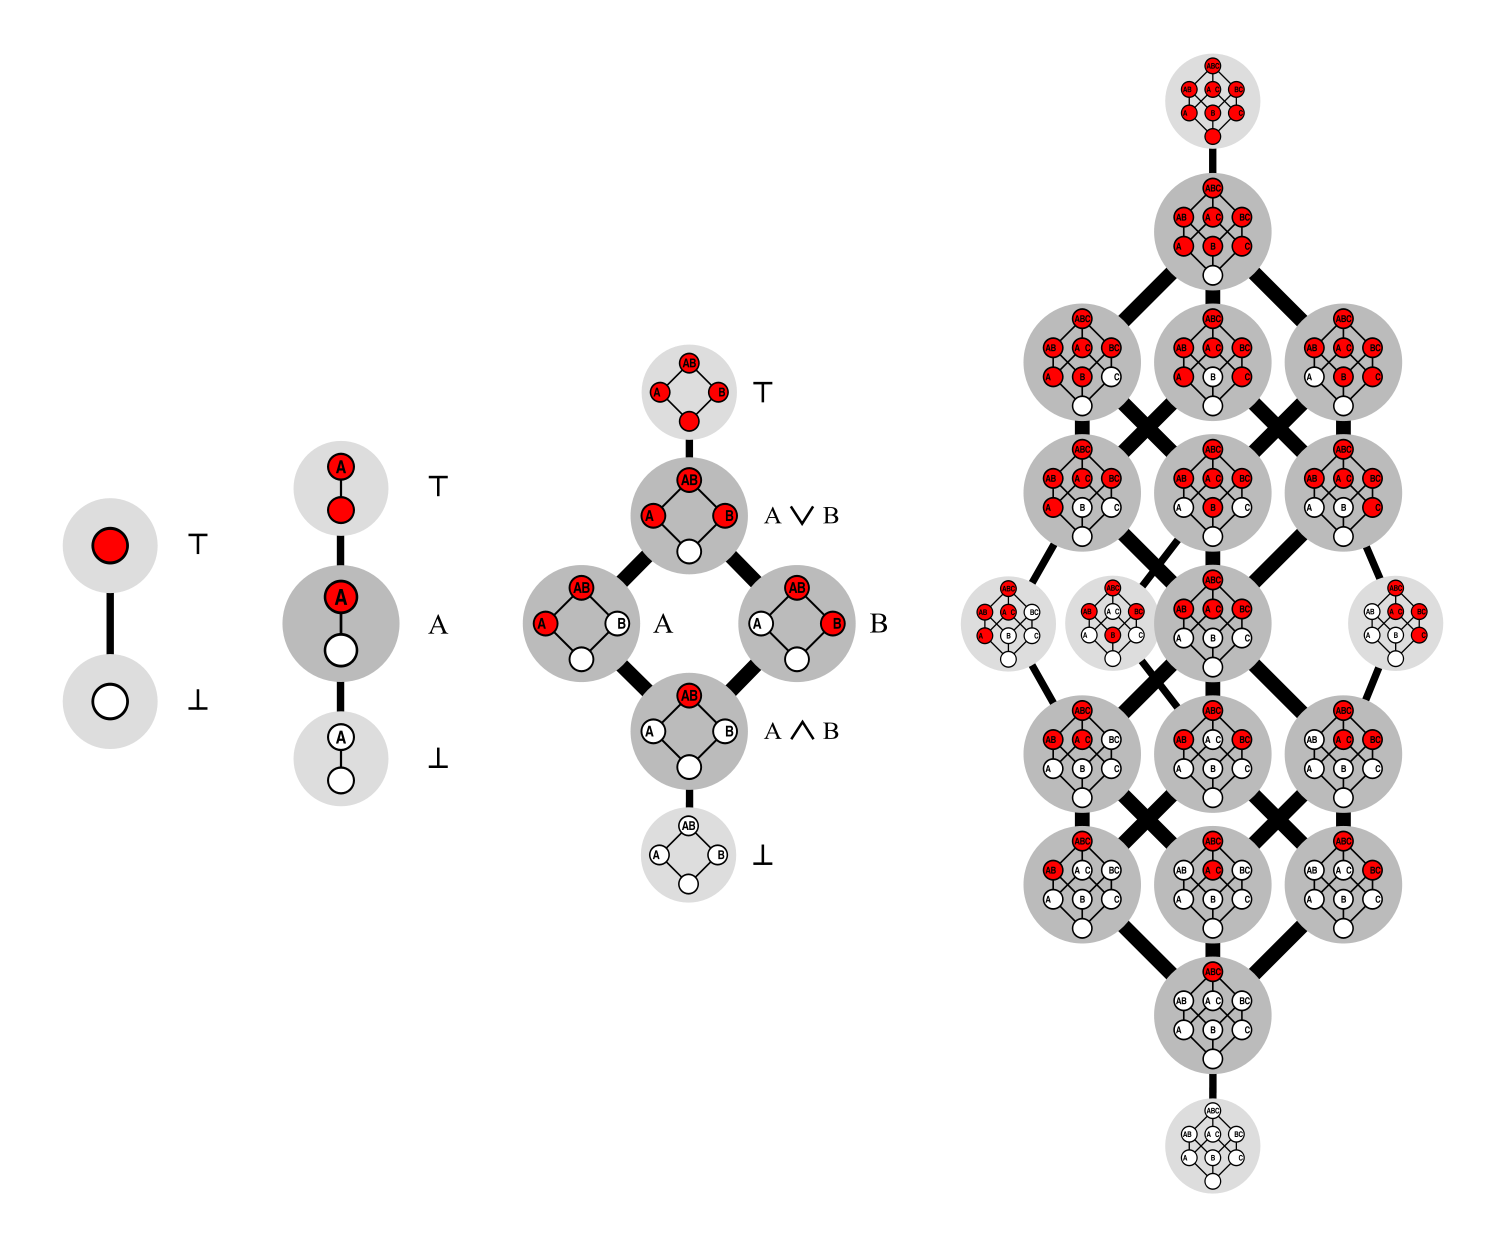
\includegraphics[scale=0.15]{kostki.png}
\caption{Wygląd kostek oraz ich "kolorowania" dla zadanej liczby Dedekinda.}
\end{figure}

\end{frame}

\subsection{Pierwszy algorytm}

\begin{frame}{Pierwszy algorytm}
\begin{block}{Pseudokod}
\begin{large}
sum = 0 \linebreak
for i = 1 to $M_{k-1}$ do \linebreak
\phantom{\texttt{\char32}\texttt{\char32}}
for j = 1 to $M_{k-1}$ do \linebreak
\phantom{\texttt{\char32}\texttt{\char32}\texttt{\char32}\texttt{\char32}}
if $M_{k-1}[i] \leqslant M_{k-1}[j]$ then \linebreak
\phantom{\texttt{\char32}\texttt{\char32}\texttt{\char32}\texttt{\char32}\texttt{\char32}\texttt{\char32}}
sum = sum + 1 \linebreak\linebreak
\phantom{\texttt{\char32}\texttt{\char32}\texttt{\char32}\texttt{\char32}\texttt{\char32}\texttt{\char32}}
$M_{k}[sum]$ =$M_{k-1}[i] \cdot M_{k-1}[j]$ \linebreak
return sum, $M_{k}$
\end{large}
\end{block}
\blfootnote{\href{http://www.ii.uni.wroc.pl/~lorys/IPL/article79-6-4.pdf}{Algorithms counting monotone Boolean functions - Robert Fidytek, Andrzej W. Mostowski, Rafał Somla, Andrzej Szepietowski}}
\end{frame}

\subsection{Drugi algorytm}

\begin{frame}{Drugi algorytm}
\begin{block}{Pseudokod}
\begin{large}
compute matrix $ r \Leftarrow u \leqslant v$ ? $r[u][v] = 1 : r[u][v] = 0 $\linebreak\linebreak
compute matrix $ re = r * r $ \linebreak\linebreak
$ sum = \sum_{i, j \in M_{k - 2}}(re[i][j])^{2}$
\end{large}
\end{block}
\blfootnote{\href{http://www.ii.uni.wroc.pl/~lorys/IPL/article79-6-4.pdf}{Algorithms counting monotone Boolean functions - Robert Fidytek, Andrzej W. Mostowski, Rafał Somla, Andrzej Szepietowski}}
\end{frame}

\section{Podsumowanie}
\begin{frame}{Podsumowanie}

\centering
\begin{Large}
Dziękuję za uwagę! \linebreak Zapraszam do dyskusji oraz pytań.
\end{Large}
\end{frame}

% \section{Bibliografia}

\end{document}
